%----------------------------------------------------------------------------------------
%	PACKAGES AND DOCUMENT CONFIGURATIONS
%----------------------------------------------------------------------------------------
\documentclass[journal]{IEEEtran}
\usepackage{amsmath} % Required for some math elements
\usepackage{hyperref}
\usepackage[table,xcdraw]{xcolor}
\usepackage{lipsum} 
\usepackage{cite}
\usepackage{graphicx} % Required for the inclusion of images
\usepackage{algorithmic}
\usepackage{array}
\usepackage{bookmark}

\interdisplaylinepenalty=2500 %Note that the amsmath package sets \interdisplaylinepenalty to 10000 thus preventing page breaks from occurring within multiline equations. Use: \interdisplaylinepenalty=2500 after loading amsmath to restore such page breaks as IEEEtran.cls normally does

\hypersetup{ %color attributes of citation, link, etc.
    colorlinks=orange,
    linkcolor=cyan,
    filecolor=gray,      
    urlcolor=cyan,
    citecolor=cyan,
}
%----------------------------------------------------------------------------------------
%	DOCUMENT INFORMATION
%----------------------------------------------------------------------------------------
\title{RESE412 - Project 1 Report \\ Sizing of a Renewable Microgrid}
\author{Daniel Eisen}
\date{\today}

\begin{document}
\onecolumn
\maketitle
\tableofcontents
%----------------------------------------------------------------------------------------
%	DOCUMENT CONTENT
%----------------------------------------------------------------------------------------
\twocolumn
\section{Introduction}
\IEEEPARstart{T}{his} project and report describes the process and presents the results of sizing a renewable energy generation solution for a relatively isolated small residential settlement. After the location and environmental circumstance was characterised, an incremental analysis was undertaken with the use of Simulink simulation modelling. Each household model was first individually sized for using a nanogrid approach for both solar and wind and had their performance documented. Then for microgrid integration, two scenarios were modelled; first the distributed model of interconnected individual nanogrids then a centralised generation topology.

The goal in doing this approach is to build a greater understanding of the energy requirement of such a settlement, evaluate the comparative cost and efficacy of the various approach's in designing a long term standalone, renewable energy solution for such a community and the drawbacks/caveats and issue associated and encountered throughout. 

\section{Environmental Analysis}
In order to design the necessary to serve the settlement, influence that the environment will have must be taken into account and characterised/considered. Firstly the immediate topology and how it will affect total hours of available sun, wind obstruction via trees, and space requirements for distancing turbines, or placing solar panels.

The site chosen for this settlement is a ridge in the south-west of the Wellington region, specifically at $-41.335^{\circ}, 174.705^{\circ}$, with a planned 6 plots for residential households though this report will only look at modelling an initial settlement of size 4.
        \subsection{Topological Discussion}
        \begin{figure}[h!]
                \centering
                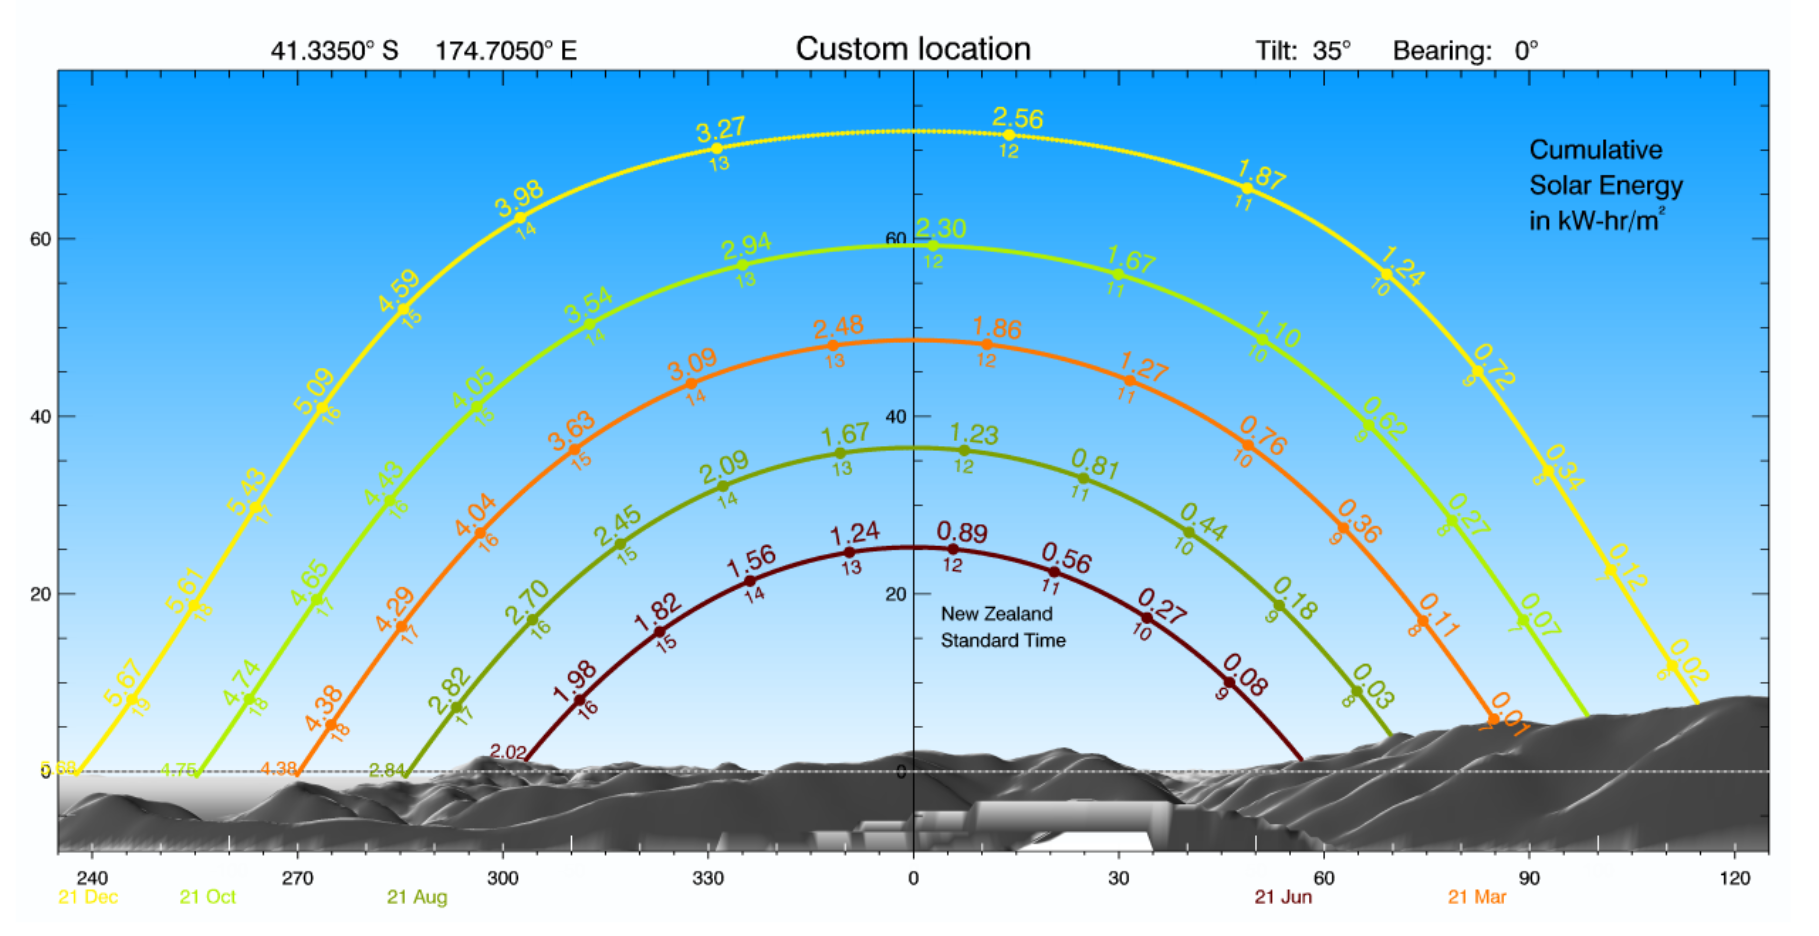
\includegraphics[width=0.75\linewidth]{fig/niwa_solarview.png}
                \caption{NIWA SolarView of Location}
                \label{solarview}
        \end{figure}

        The site is a flat, treeless ridge so environmental obstructions, see appendix \ref{ap:location}, to wind or solar are completely minimal and the only considerations that would need to be taken into account are placement during construction; concerning panel array placement (if not rooftop) and staggering turbine as to have them out of line with each other.

        Figure \ref{solarview} shows the the solar obstruction mapping from the north bearing. I can be seen that the rise time in summer is cut off to just before 6am, but more importantly in winter when solar irradiance is at a premium there is practically no restriction is the time between rise/set that there should theoretically be available sun. 

        These two observations; the lack of trees and minimal solar occluding hills/surrounding elevations indicates that investigations into the viability of both solar and wind as avenues of usable generation is feasible.
        
        \subsection{Solar Resources}
        NIWA provides the online tool SolarView\cite{solarview}. This was used to obtain detailed weather/environmental data about a specific location, taken from averaging past 25 years of collected data into a 'nominal' years worth of representative information. This requires the input of the locals coordinates and the indented panel tilt in degrees. By default SolarView will use the latitude but using an more optimal equation (from lat 25-50) \ref{tilt} a percentage of optimum capture of 71.1 can be achieved. For this location this is $\approx 35^{\circ}$.
        \begin{equation}
                Array_{tilt} = |lat|*0.76 + 3.1
                \label{tilt}
        \end{equation}

        From SolarView's provided data, the tilted irradiance is representative of what solar energy will be available to the installation for capture. From the years worth of data, a week was chosen to be the basis on which to characterise and size the nano/microgrids. This week is required to be 'averagely bad', meaning should not be an outlier in terms of terrible solar irradiance, having low average $W/m^2$ and a mix of slightly better and worse days. By sizing the installation for performing well in winter it can be taken for granted to work above specification across all the better months of the year.

        \begin{figure}[h!]
                \centering
                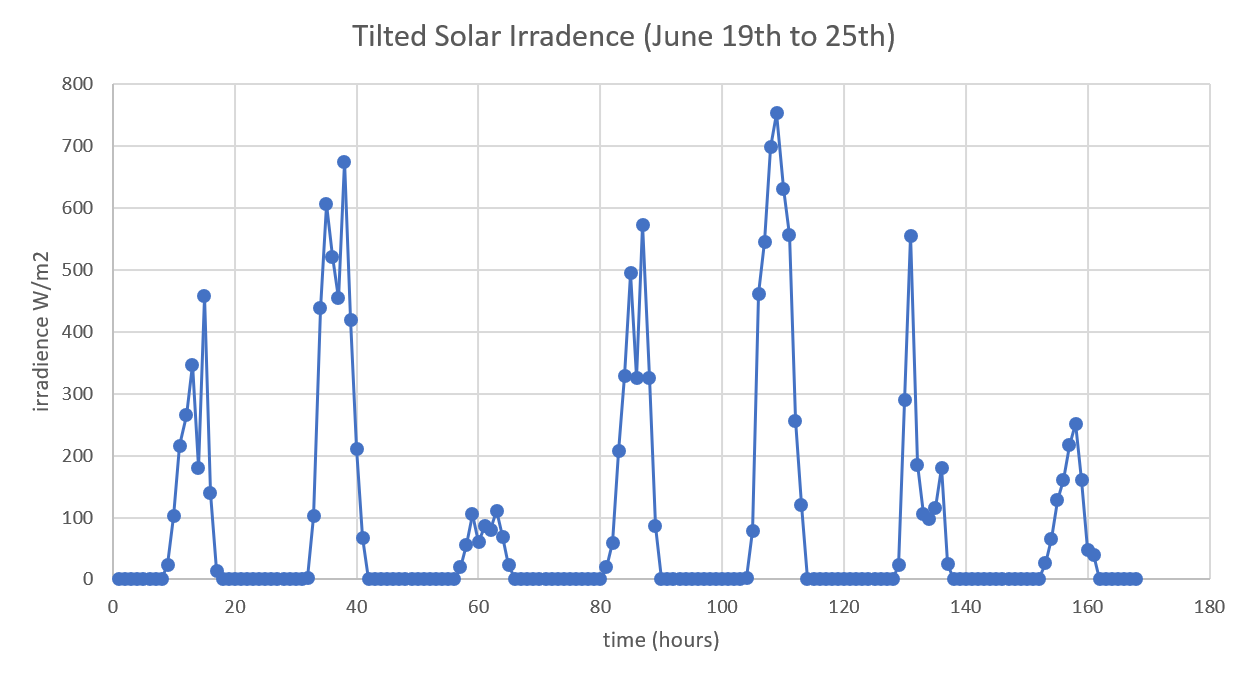
\includegraphics[width=0.75\linewidth]{fig/solar_irad.png}
                \caption{Solar Irradiance for chosen week}
                \label{solarweek}
        \end{figure}

        Taken the winter solstice (21 June) as a starting point, the 4 weeks of available solar irradiance surrounding were look over and 7 consecutive days were selected to meet the above defined specification. Resulting in the 7 days from the 19st to the 25th of June to represent an average week providing higher and lower days of available irradiance. Figure \ref{solarweek} shows this week, observing the low max irradiance of approximately $700W/$ and the spread of very low, medium and relatively higher days throughout the 7 days. This should provide a good basis for sizing a resilient installation.


        To quantify the solar resource into a singular usable number, this weeks data was transformed peak solar hours. Ie how many equivalent hours per day can the solar panel expect to receive the peak $1000 W/m^2$ of solar irradiance. This can either be done for each days average then taking the median, or by averaging the week then taking the peak solar hours. The latter was done in this case, doing either way yields very similar results, to result in \textbf{2.14 hrs}.

        \subsection{Wind Resources}
        To contrast and compare to the solar resource, the wind resource of the area is also taken into account. For ease of comparison the same week was chosen to use wind speed data from. 
        \begin{figure}[h!]
                \centering
                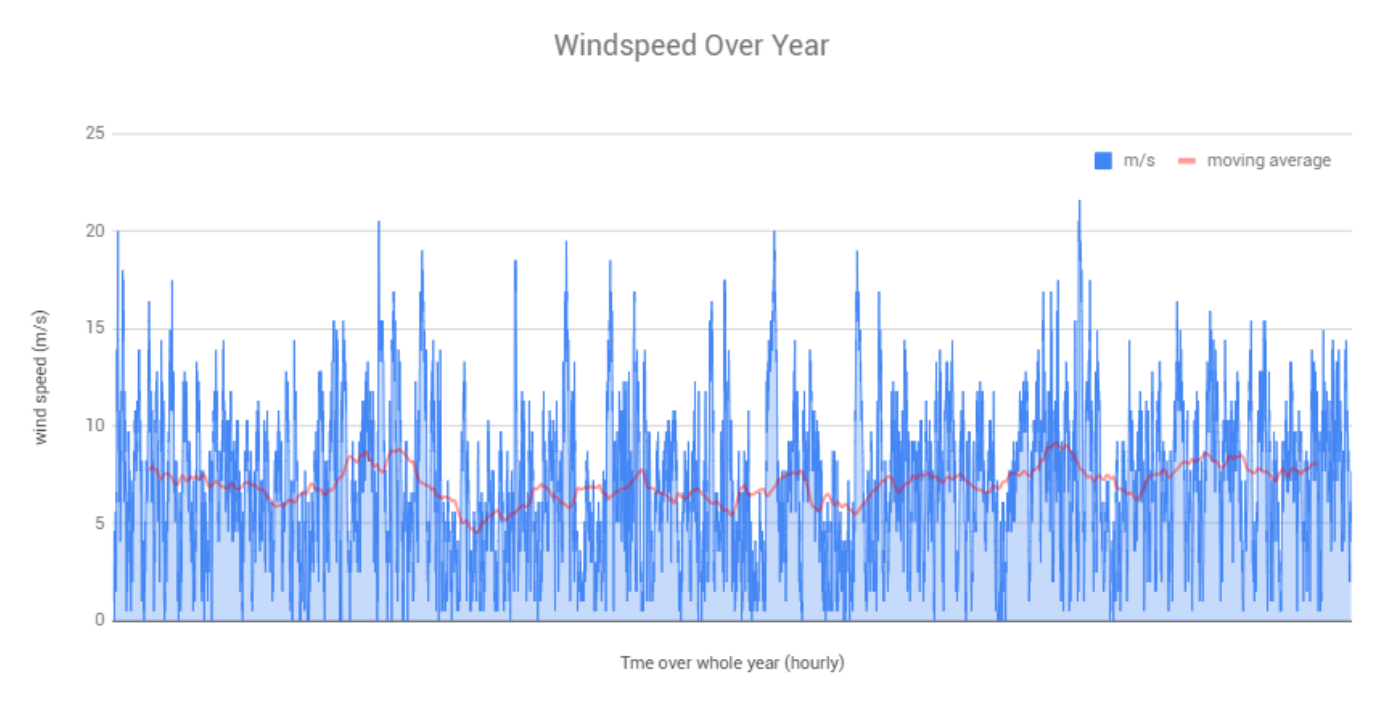
\includegraphics[width=0.75\linewidth]{fig/yearws.png}
                \caption{Year worth of windspeed}
                \label{yearwind}
        \end{figure}
        While this may not at first seem to be selected with the same rigour as the solar irradiance by observing the years data, see Figure \ref{yearwind}, it can be seen that for this location the windspeed level does not have any large scale cycling, possibly even a slight dip in the winter months maybe due to lower driving solar energy, so it can be treated as a fair and representative week for the year.
        
        \begin{figure}[h!]
                \centering
                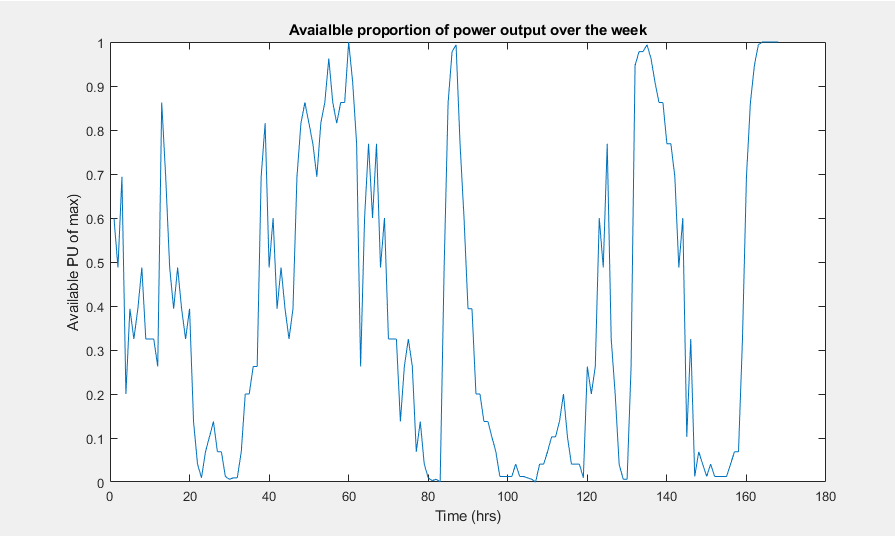
\includegraphics[width=0.7\linewidth]{fig/windPU.png}
                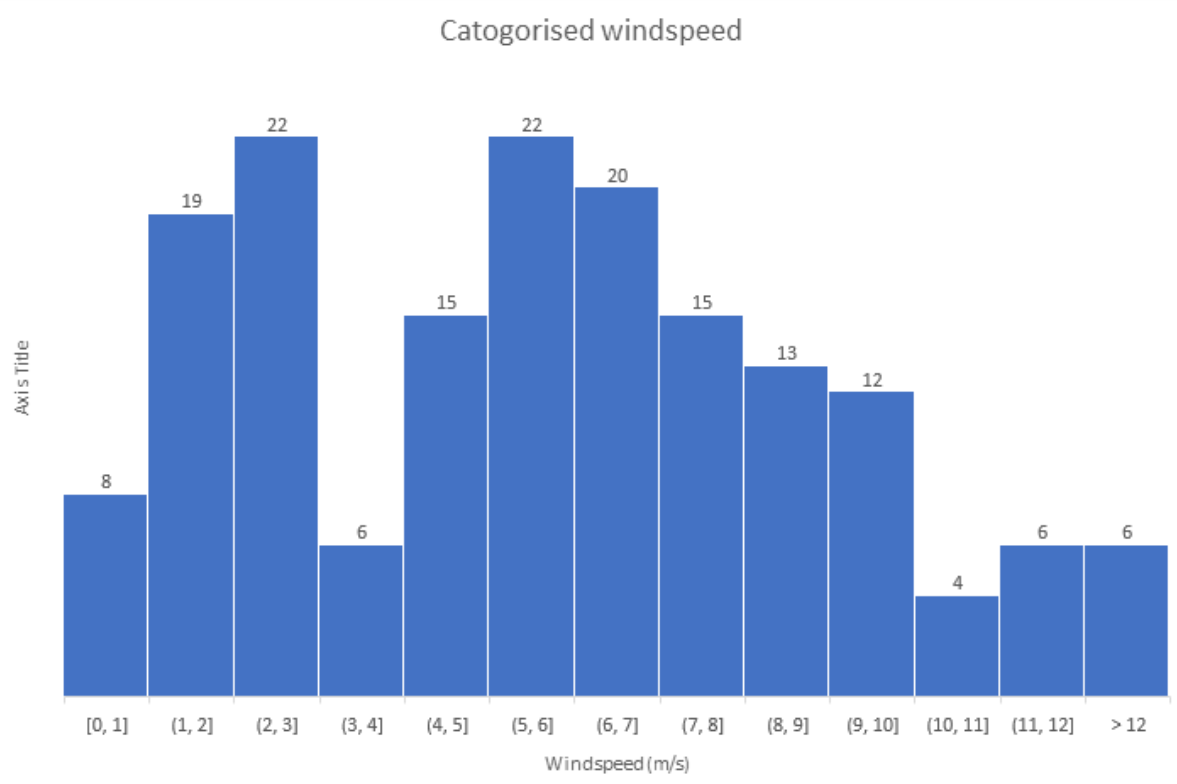
\includegraphics[width=0.7\linewidth]{fig/catorgws.png}
                \caption{Available turbine PU and windspeed histogram}
                \label{wind}
        \end{figure}
        In evaluating the wind resource the non linear and the turbine response has a maximum cap on its output at windspeeds greater than $12m/s$. See appendix \ref{ap:wind}. Figure \ref{wind} shows (right) the gross windspeed data binned into a histogram squashing speeds over-saturation and left is the result of running an interpolation of the data to the turbine response curve to retrieve its proportion of maximum power output over the week $(0.0 \rightarrow 1.1)$. Similarly to the peak sun hours previously discussed, this was used to determine the single value evaluation of the available wind resources. Summing the resulting vector and dividing by the number of days analysed results in a value of \textbf{9.43} equivalent hours of maximum turbine output. 
        
\section{Household Load Analysis}
Each home was characterised by simulating a week’s worth of usage, and averaging the integrated power usage to obtain a average daily usage, ie their energy consumption, scaled to kWhs. This way it accounts for slight variation across the days of the week.

\begin{table}[h!]
        \begin{center}
        \begin{tabular}{ll}
                \textbf{House} & \textbf{daily usage (kWh)}   \\
                \rowcolor[HTML]{C6EFCE} 
                2 & 17.88 \\
                \rowcolor[HTML]{FFEB9C} 
                3 & 19.78 \\
                \rowcolor[HTML]{FFC7CE} 
                4 & 16    \\
                \rowcolor[HTML]{BDD7EE} 
                5  & 39.59                       
        \end{tabular}
        \end{center}
\caption{Daily load requirements per household}
\label{tab:load}
\end{table}

\begin{figure}[h!]
        \centering
        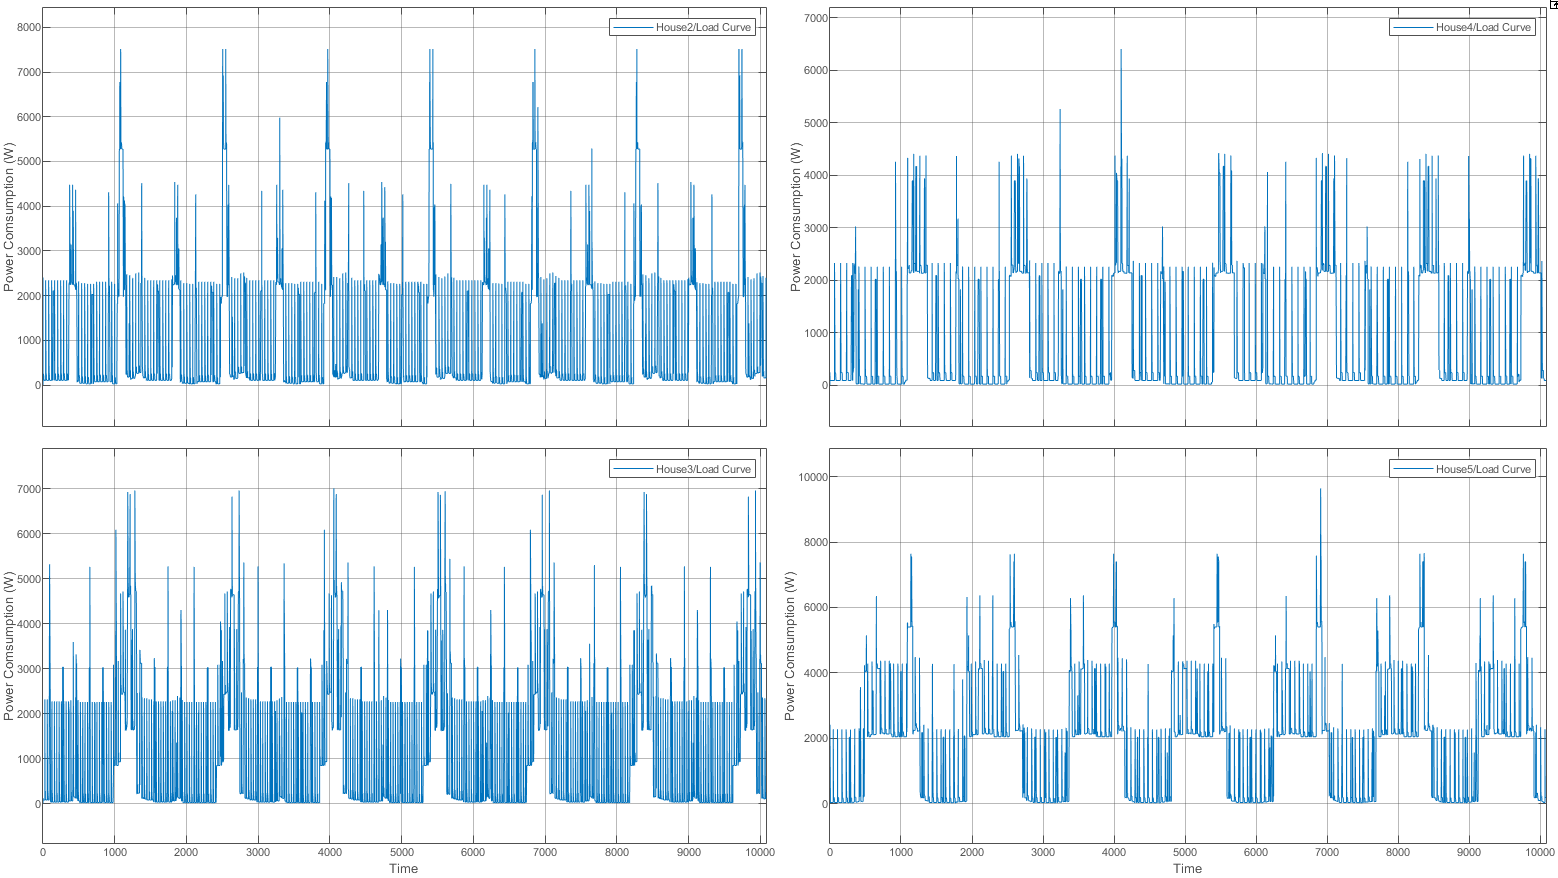
\includegraphics[width=0.75\linewidth]{fig/houseloads.png}
\caption{Household load}
\label{fig:load}
\end{figure}

The results of these simulation are shown above: Table \ref{tab:load} outlines the daily energy use per household as averaged over the week of simulation, indicating the necessity of individually sized solutions for each such that the nanogrids maximise they're efficiency, i.e. to avoid under/over-production.
These total usage values allow for the initial sizing of the generation, but without a look at the variation across daily usage in order to build an idea of how to smooth misalignment of generation to consumption with the right combination of generator and storage capacity. 
Some initial observations that will factor into the sizing are for example; house 5s much higher base load but also its consistency so high overlap with the solar generation period. Also house 4 with its majority consumption after the peak available sun, which will affect the needed storage in comparison to similar, but distributed loads.
\section{Nano-grid Sizing}
For sizing the nanogrid installations, the quantified available resources and the estimated household loads are used to calculate initial parameters for both a solar and a wind centric systems.
To meet the requirement of a necessarily performant nanogrid the system must be able to meet at least 95\% of the its load requirement and ideally greater than 97\%.   
 These are then evaluated in a via a Simulink model to evaluate how they perform against the preventing define metric, with the performance parameters being the \% of unmet load.
 From this evaluation the parameters are modified if necessary to better meet the requirements and revaluated.   

\textit{For full table see appendix \ref{ap:initnanosize}.}
        \subsection{Initial Estimates}
                \subsubsection*{Storage}
                For initial testing, the BMS storage is set to a minimum capacity allowing for a days worth of autonomy, ie matching the kWh load of each house to a Ah capacity bank at 240V. This should provide the minimum protection against poor generation days, but this is assumes a large overlap of generation and consumption.\\

                It must be notes that the costing of 5.6 \$/Ah provided\cite{DANNYB} was incorrect and based on price of capacity for 12V battery systems. So pricing following are inaccurate though process and comparison methodology are sound the absolute concluding values are inaccurate due to this.
                \begin{itemize}
                        \item House 2: 74.5Ah
                        \item House 3: 82.42Ah
                        \item House 4: 66.67Ah
                        \item House 5: 164.96Ah
                \end{itemize}


                \subsubsection*{Photovoltaics}
                To make initial estimate for sizing system, the  characterised available resources is used. Taking the daily usage and dividing the peak hours to get an initial panel wattage size for each home. This is used as a starting point that was evaluated via the simulations.
                \begin{figure}[h!]
                        \centering
                        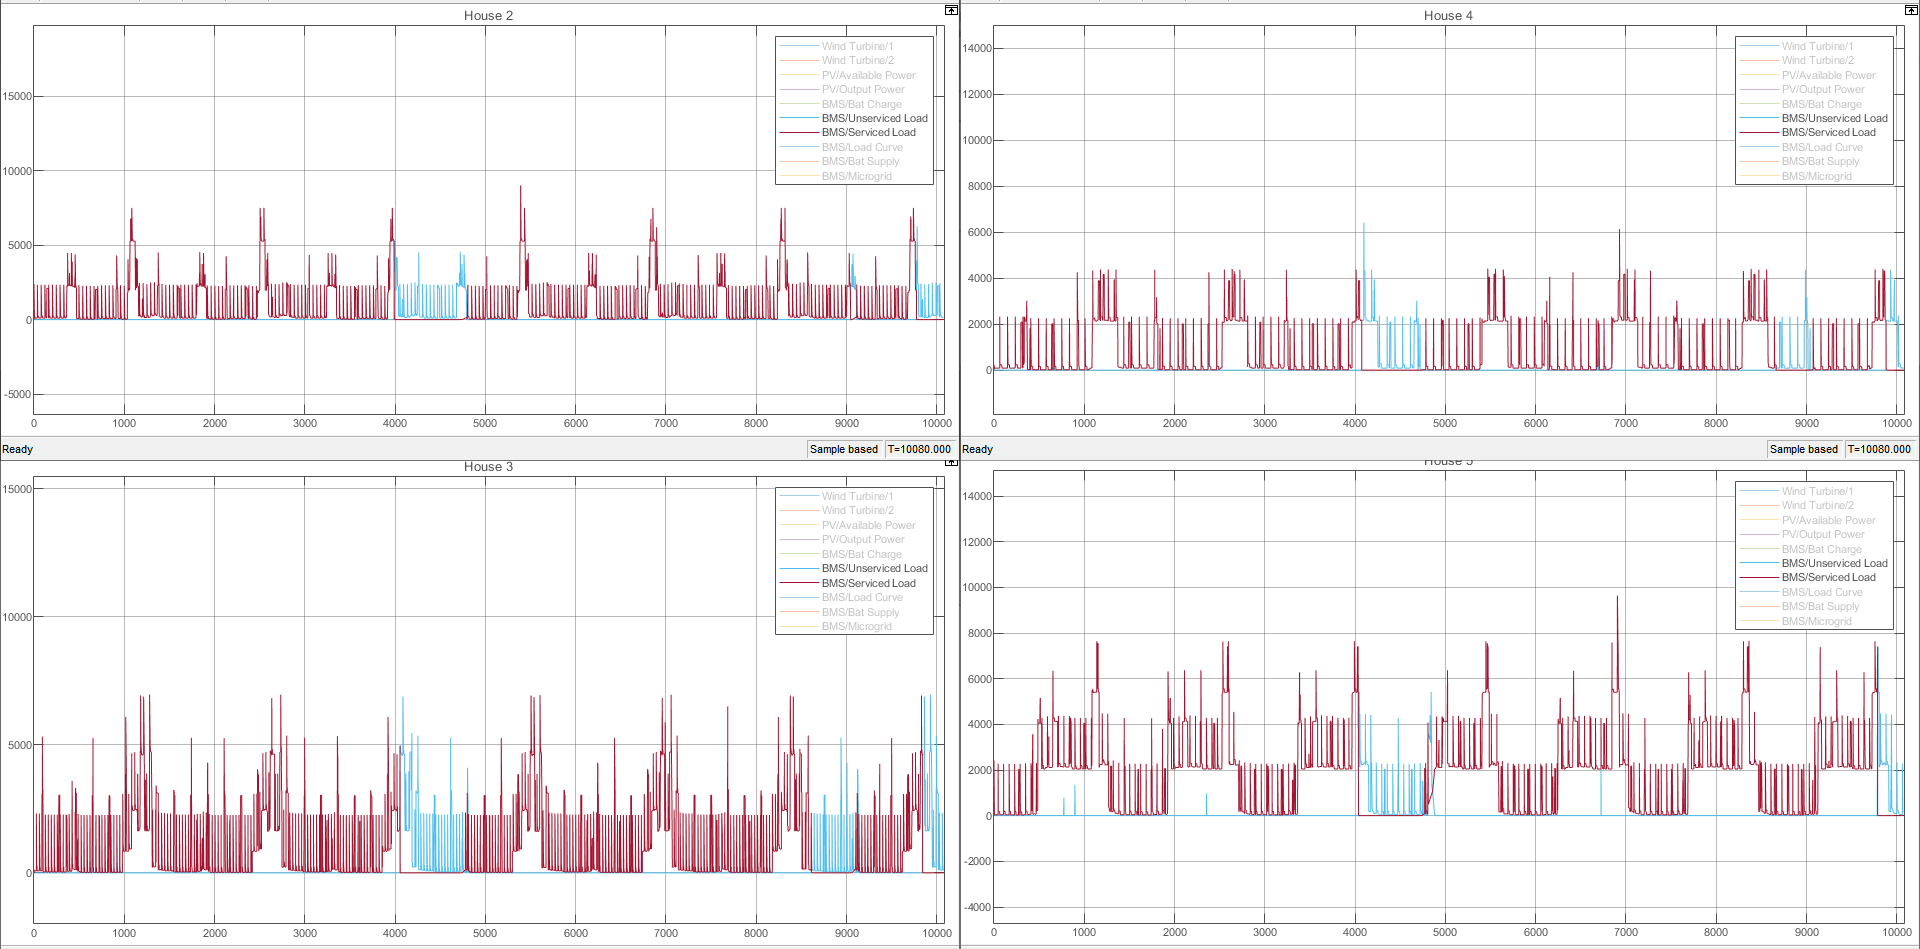
\includegraphics[width=0.7\linewidth]{fig/init_solar_load.png}
                        \caption{Serviced and Unserviced Load}
                        \label{fig:solar_init}
                \end{figure} 
                Figure \ref{fig:solar_init} shows the failure of the initial solar system to provide requirement load threshold in all cases over a week of simulation. This is quantified as follows:

                \begin{table}[h!]
                        \centering
                        \begin{tabular}{|l|l|}
                        \hline
                        \textbf{House} & \textbf{unserviced (\%)} \\ \hline
                        2              & 12.68                    \\ \hline
                        3              & 15.73                    \\ \hline
                        4              & 15.84                    \\ \hline
                        5              & 6.01                     \\ \hline
                        \end{tabular}
                        \end{table}

                \subsubsection*{Wind Turbine}
                As with the photovoltaic sizing, the requirement is divided by the available output from the turbine to reach daily consumption and simulations rerun with the same requirements.

                \begin{figure}[h!]
                        \centering
                        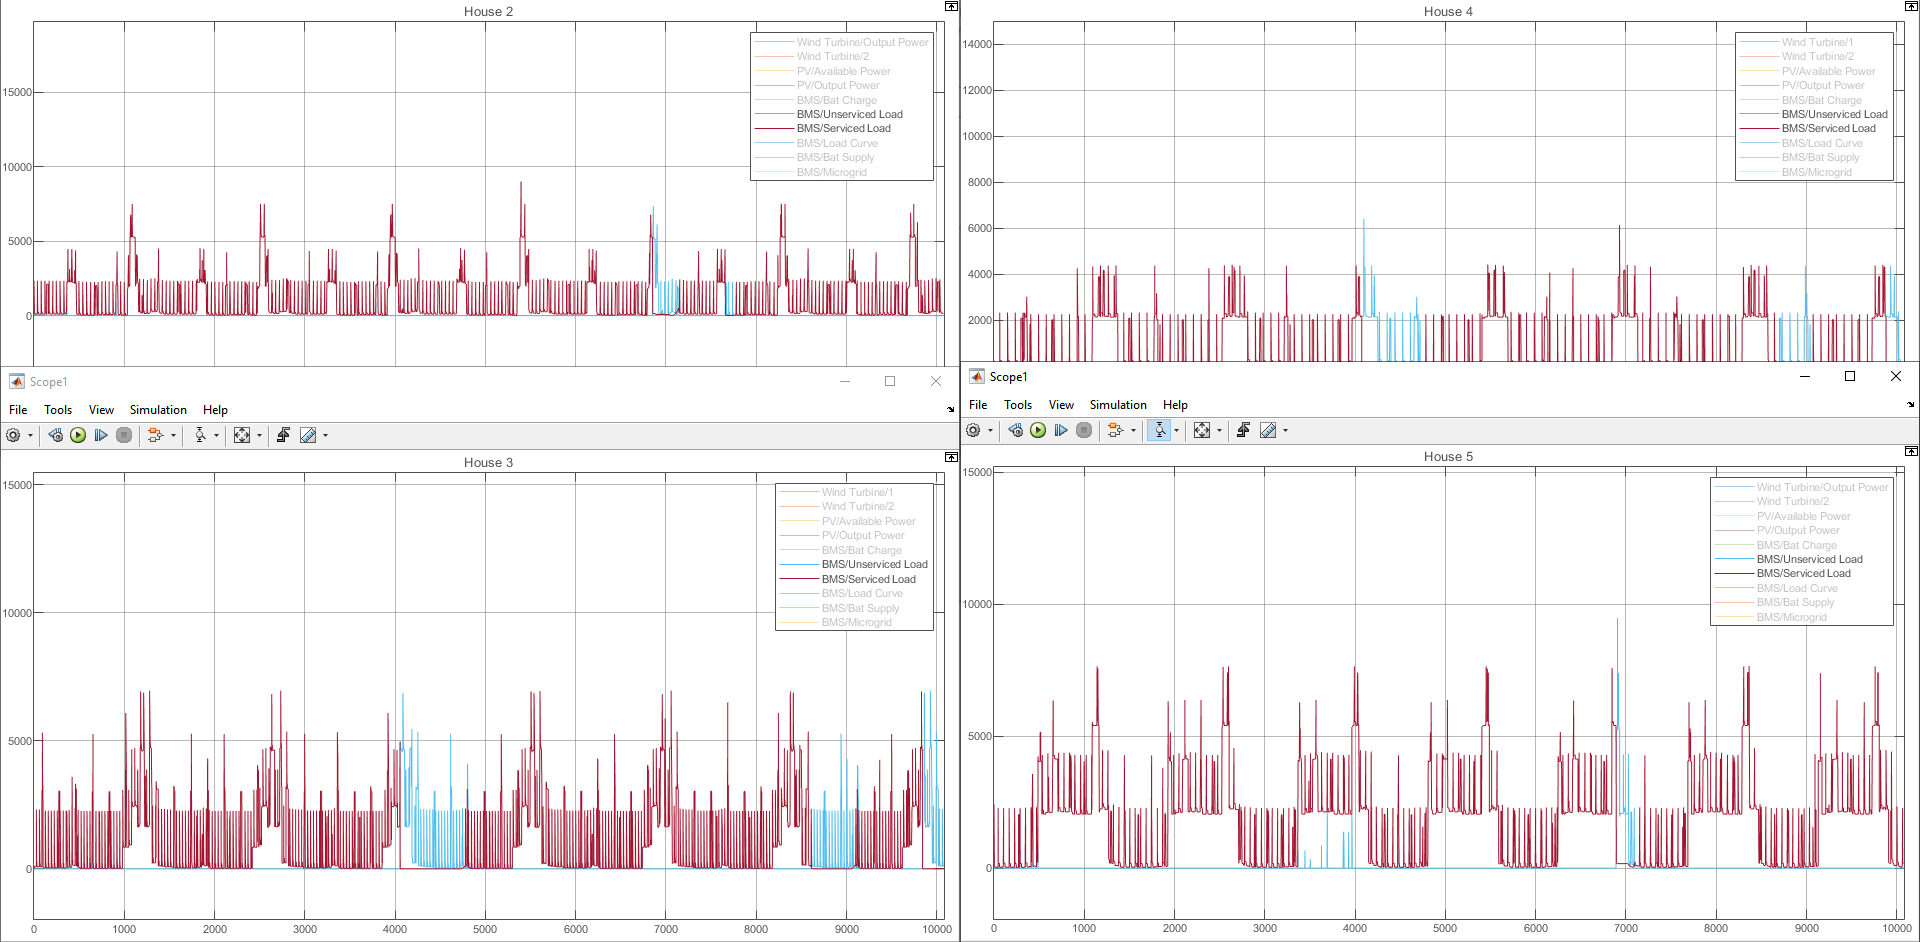
\includegraphics[width=0.7\linewidth]{fig/init_wind_load.png}
                        \caption{Serviced and Unserviced Load}
                        \label{fig:wind_init}
                \end{figure} 

                These initial sizing's for the turbine based system meet the requirements for both houses 2 and 5. As the figure \ref{fig:wind_init} shows, this occur with battery drainage in the evenings of high load, and 2 days of low generation.

                \begin{table}[h!]
                        \centering
                        \begin{tabular}{|l|l|}
                        \hline
                        \textbf{House} & \textbf{unserviced (\%)} \\ \hline
                        2              & 4.672                    \\ \hline
                        3              & 6.8                      \\ \hline
                        4              & 7.906                    \\ \hline
                        5              & 2.596                    \\ \hline
                        \end{tabular}
                        \end{table}
                
                

        
        \subsection{Simulation and Meeting Final Requirements}
        In order to meet the difference between the stated requirements for these systems and the results of the initially calculated parameters the generation power output and/or storage must be increased.

        Due to the effect of the the previously mentioned battery costing mistake, and the fact that the final costing will double the battery capacity of what was simulated to ensure longer lifetime (i.e. mitigating deep discharge wear), this stage of optimising component values limited the battery capacity to 1.5 times the daily energy requirements per household (though this limit was never met).

        The process taken was to initially round all calculated values up to the nearest whole or whole plus one half value and revaluate. The battery level and its failure (empty) was observed to motivate capacity increase and the available vs utilised power of the generation was used to motivate power rating increase of both the panels and turbines. 

        This process was iterated upon, but did not required a large amount of retuning (average achievement of requirements with 3 simulations), until a preferred level of satisfaction is achieved.  
        \subsubsection*{solar}
        Solar required the larger increase of both photovoltaics and storage to all houses.
        \begin{table}[h!]
                \begin{tabular}{llll}
                House & PV (kW) & storage (Ahr) & unserviced (\%) \\
                2     & 10      & 95            & 3.6             \\
                3     & 12      & 100           & 2.6             \\
                4     & 10      & 85            & 3.64            \\
                5     & 20      & 180           & 1.9            
                \end{tabular}
                \end{table}
        \subsubsection*{wind}
        Wind required only small rounding up of calculated values for 2,5 and small increases for the other two. House 4 required relatively large battery due it tail heavy load requirements.
        \begin{table}[h!]
                \begin{tabular}{llll}
                House & Turbine (kW) & storage (Ahr) & unserviced (\%) \\
                2     & 2            & 80            & 2.68            \\
                3     & 2.6          & 95            & 3.2             \\
                4     & 1.8          & 85            & 4.031           \\
                5     & 4.5          & 165           & 1.79           
                \end{tabular}
                \end{table}

        With this approach the requirements were met with a reasonable solution. How reasonable these were will be compared and determine following.
        
        \newpage
        \subsection{Costing}
                \subsubsection*{solar}

                The final total cost for the 4 sized solar nanogrids is \$140,352.00.
                
                \begin{table}[h!]
                        \begin{tabular}{|l|l|l|l|}
                                \hline
                                \textit{\textbf{House}} & \textit{\textbf{PV cost (\$)}} & \textit{\textbf{storage cost (\$)}} & \textit{\textbf{Total cost (\$)}} \\ \hline
                                2                       & \$            26,000.00        & \$          1,064.00                & \$    27,064.00                   \\ \hline
                                3                       & \$            31,200.00        & \$          1,120.00                & \$    32,320.00                   \\ \hline
                                4                       & \$            26,000.00        & \$             952.00               & \$    26,952.00                   \\ \hline
                                5                       & \$            52,000.00        & \$          2,016.00                & \$    54,016.00                   \\ \hline
                        \end{tabular}
                \end{table}
                \subsubsection*{wind}

                The final total cost for the 4 sized wind nanogrids is \$77,136.00.
                \begin{table}[h!]
                        \begin{tabular}{|l|l|l|l|}
                        \hline
                        \textit{\textbf{House}} & \textit{\textbf{turbine cost (\$)}} & \textit{\textbf{storage cost (\$)}} & \textit{\textbf{Total cost (\$)}} \\ \hline
                        2                       & \$            13,280.00             & \$             896.00               & \$    14,176.00                   \\ \hline
                        3                       & \$            17,264.00             & \$          1,064.00                & \$    18,328.00                   \\ \hline
                        4                       & \$            11,952.00             & \$             952.00               & \$    12,904.00                   \\ \hline
                        5                       & \$            29,880.00             & \$          1,848.00                & \$    31,728.00                   \\ \hline
                        \end{tabular}
                        \end{table}
        \subsection{Wind vs Sun}
                        In this location it has been seen in previous sections that wind is a more stable and more available resource than solar, can provide a better load satisfaction per household for a smaller installation, and cost significantly less. 

                        Turbine generation design is relatively more complex than that of a solar installation. With placement key in obtaining the optimal output these model rely on, ie in avoiding turbulent flow, reduced windspeed and wind blockage from not just the households but the other turbines.  

        \subsection{Notes on Hybrid}
        It was outside the scope of time for this project to properly analyse a hybrid (both wind and solar generation) approach so it cannot comment on the possible efficacy and cost savings. It can however offer the consideration that a duel generation approach can offer mitigation to the problem of non overlapping generation and consumption periods, with the capability for each source to hand off as they wane to either direct use, or storage charging. 




\subsection{Final Nanogrid}
The final nanogrid design that will be carried through to the sizing of the microgrids are the wind turbine based sizing as fully outlined in appendix \ref{ap:finalnanosize}.

\section{Microgrid}
        \subsection{Distributed}
        The distributed microgrid allows for the sharing of generation between the households and a model (\ref{ap:models}) was constructed from the connection of the previously sized and evaluated wind turbine based nanogrid installations. These were connected via line models to account for resistant losses and run with the same wind resource and component sizing to evaluate if the interconnection served to balance load losses between generation sights and improve the settlement performance as a whole.

        \begin{figure}[h!]
                \centering
                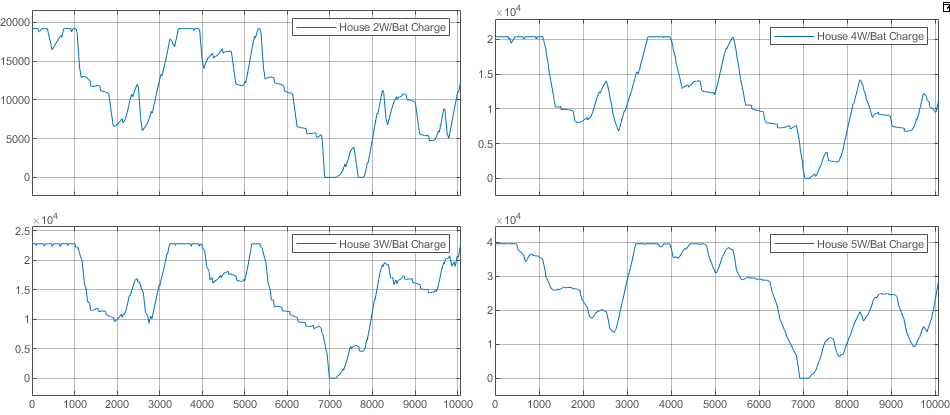
\includegraphics[width=0.7\linewidth]{fig/distrib_bat.png}
                \caption{Household battery capacity in distributed microgrid}
                \label{fig:distrib_bat}
        \end{figure} 

        \begin{figure}[h!]
                \centering
                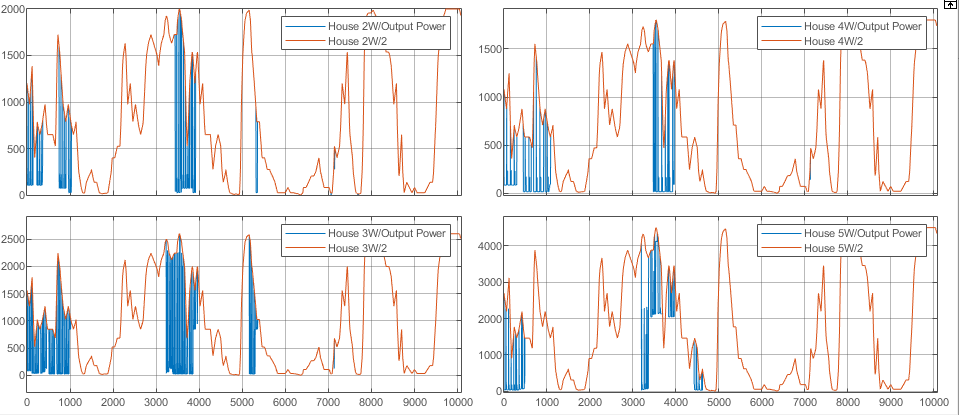
\includegraphics[width=0.7\linewidth]{fig/distrib_gen.png}
                \caption{available energy use per household}
                \label{fig:distrib_gen}
        \end{figure} 

        \begin{figure}[h!]
                \centering
                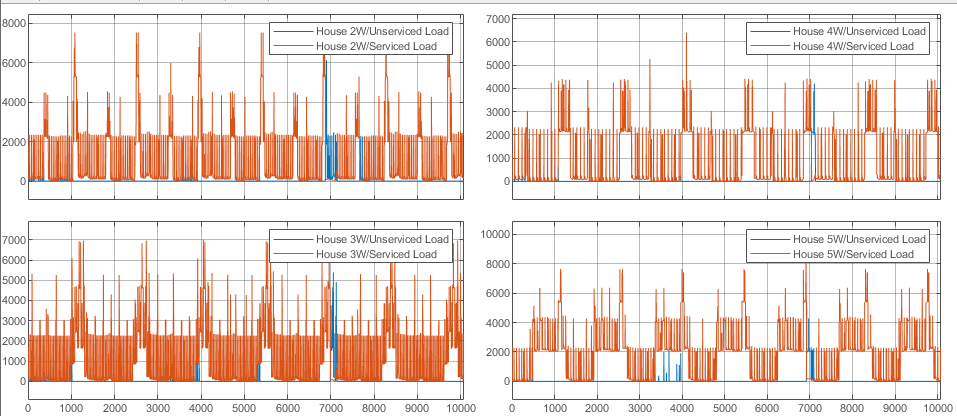
\includegraphics[width=0.7\linewidth]{fig/distrib_load.png}
                \caption{load served and unserved per household}
                \label{fig:distrib_load}
        \end{figure} 

        \begin{figure}[h!]
                \centering
                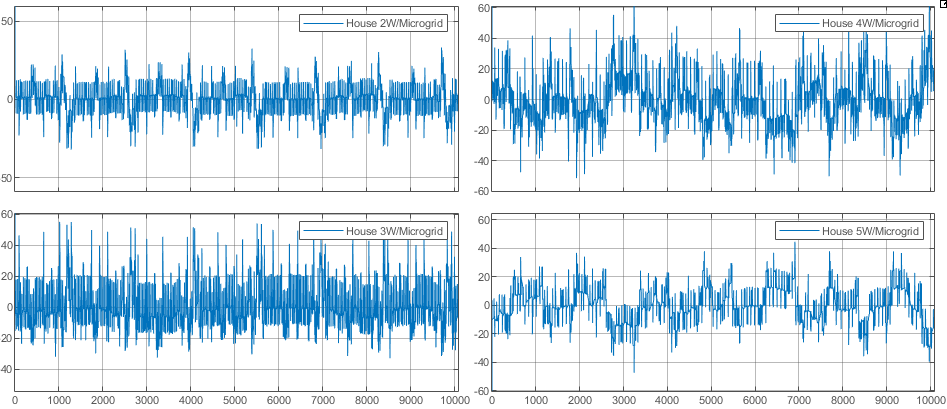
\includegraphics[width=0.7\linewidth]{fig/distrib_micro.png}
                \caption{Shared power between households in microgrid}
                \label{fig:distrib_micro}
        \end{figure} 

        For full tabulated results see \ref{ap:micro}:
        
        To summarise the results the interconnection, reduced the unserved load of house 4 by 1\$ (from 4 to 3) with little impact on the other 3 houses. All are still within threshold. 
        As figures \ref{fig:distrib_load},\ref{fig:distrib_micro} show, there a large amount to power exchange occurring in houses 4 and 5 relative to 2 and 3, and this is expended as they are physically closer, 4 has a more uneven load destruction and 5 has a large generation base. 
        Its total cost is excluding line laying cost, and is identical to that outlined in the nanogrid sizing: \$77136.00 and has an averaged unserviced load of 2.67\%. 

        \subsection{Centralised}
        Modelling the Centralised topology is simpler. As a starter the already sized parameters and summing them into a singular turbine and battery system installation, connected to all houses as a whole. 

        \begin{table}[h!]
                \begin{tabular}{lll}
                Turbine (kW) & storage (Ahr) & unserviced (\%) \\
                10           & 400           & 1.982          
                \end{tabular}
                \end{table}

        This yielded initial unserved load of less than 1\% so it provided the ability to reduced the system parameters to a final value of a 10kW turbine and a 400Ah battery bank to deliver a $<2\%$ unserviced load to the settlement, as well as reducing the microgrid cost by \$7000.00.

        \begin{figure}[h!]
                \centering
                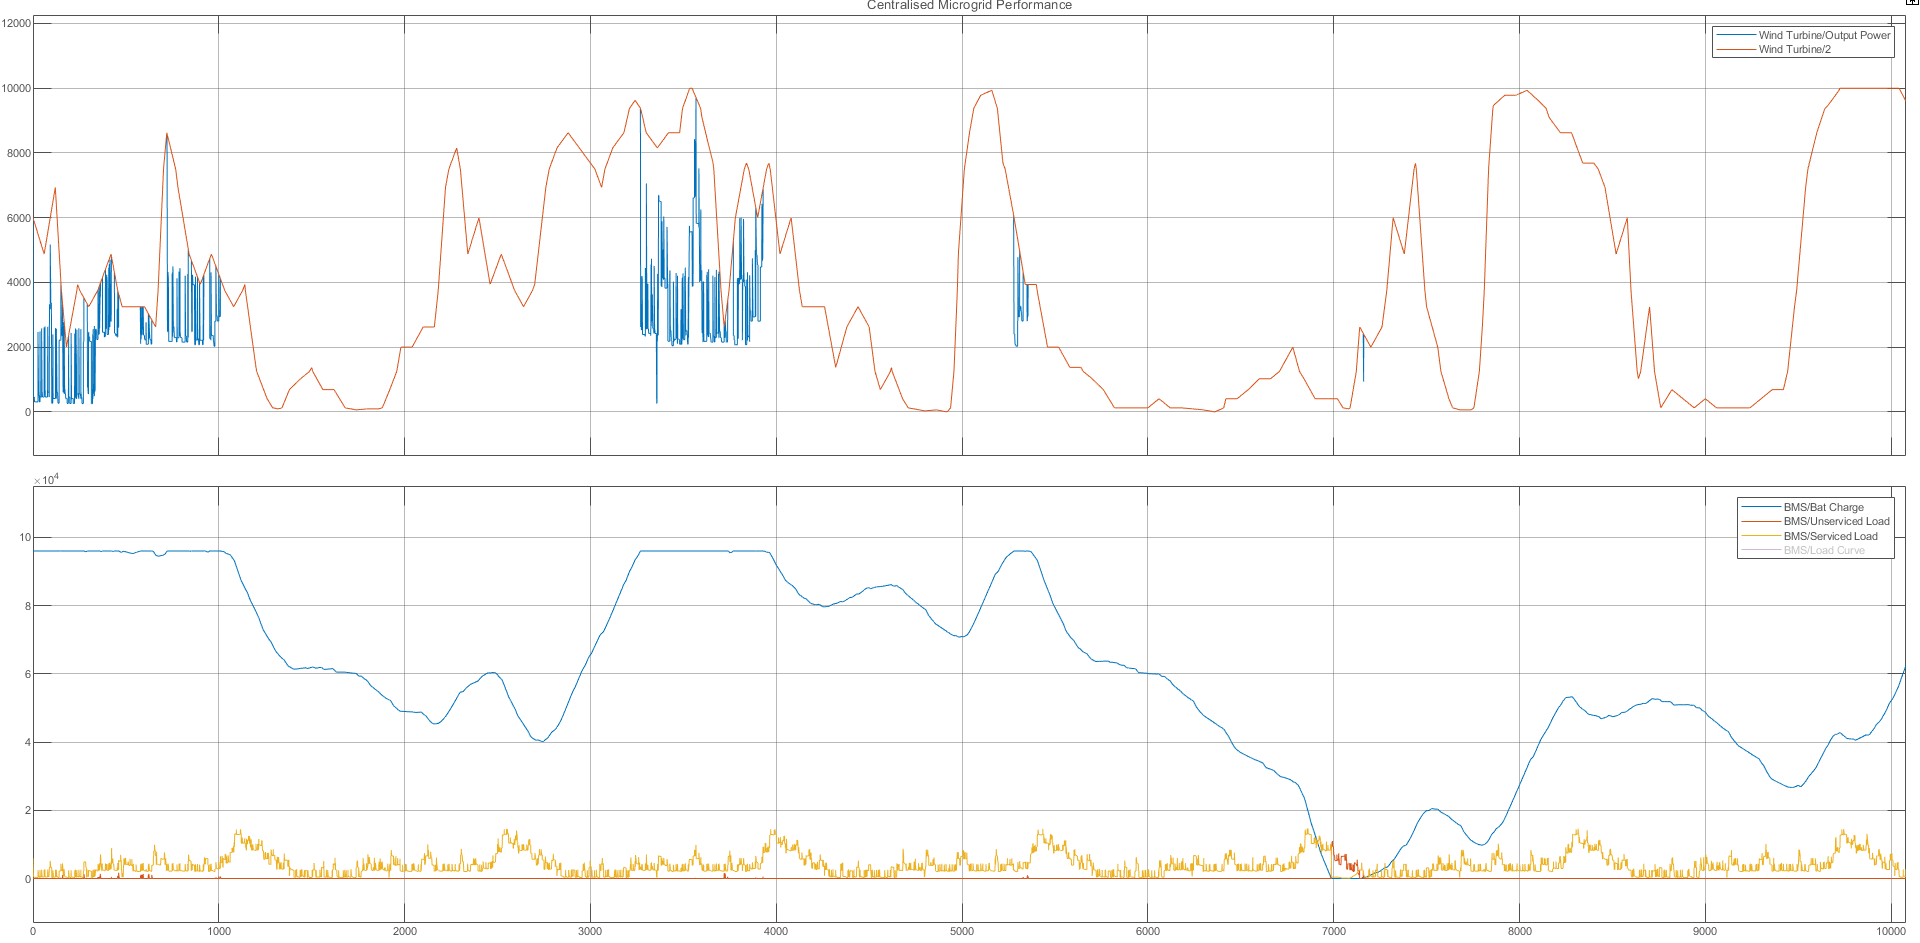
\includegraphics[width=0.7\linewidth]{fig/central_results.png}
                \caption{Full characteristics of the Central Microgrid.}
                \label{fig:central_micro}
        \end{figure} 

        Notes: The simulation shows a reduction in total load requirements be approximately 3kWh. This is may be attributed to the elimination of multiple BMS's but is likely a flaw in the simulation or the constructed model.

\section{Reflecting on the Process}
The process steps in theory result in a good hierarchical approach in tackling the problem/puzzle of sizing  renewable energy generation system. With each sequential macro-step laying the necessary foundation and information/data collection needed to complete the next and I found my self very rarely back tracking into previous step other than to correct errors or confirm results.
Resource evaluation provides the data required to make initial calculations for the small scale component selection that allows for model creation and tuning of those parameters to meet the requirements. These models and parameters could then be abstracted and packaged to combined into a larger scale system for further integrated evaluation without the need to repeat step 2.

Where the process did falter is where most do, and that is the toolset. Mostly due to errors and inconsistencies in the simulating/modelling stage of the process was it held up the most. Adding line losses sometimes provided expected results but sometimes reduced the over all load (centralised).

\section{Conclusions and Recommendations}
From this report it can be concluded that the area has a more valuable wind resource across a more of the year, than the availability of cognisant and easily (and more cost effectively) utilisable solar energy. The simulations also draw initial results indicating that for this size of settlement as centralised generation method yields a more efficient and robust solution than that of a small distributed network of generation. One must take these results however as preliminary and as a starting point for further investigation/verification, as the process possesses potential flaws and definite mistakes that need to be addressed.  

To the client this report recommends, based on the conclusions of the process, that the location is sufficiently able to support a renewable, off-grid, and energy self-sufficient settlement; and would recommend that over a grid connection due to upfront cost.
Areas that are worth investigation for implementing this solution are wind turbine based centralised generation system at the specified site.

\section{Reflecting on the Project}
The project itself, barring the bugs and issues faced in the simulations, was genuinely captivating and shed a great deal of light on the theory taught in class. I found the process streamlined just enough, thanks in huge part due to the premade models, to allow for quick entry but still provided the depth and complexity needed to spur the need for a critical approach in completing it. 


\newpage
\onecolumn
\appendices
        \section{Initial Nano Tables}
        \begin{table}[h!]
                \begin{tabular}{|l|l|l|l|l|l|l|l|l|}
                \hline
                \rowcolor[HTML]{C0C0C0} 
                \multicolumn{9}{|c|}{\cellcolor[HTML]{C0C0C0}\textit{\textbf{Initial   Solar}}}                                                                                                                                          \\ \hline
                \textbf{House} & \textbf{daily usage (kWh)} & \textbf{Peak Hrs} & \textbf{PV (kW)} & \textbf{PV cost (\$)}   & \textbf{storage (Ahr)} & \textbf{storage cost (\$)} & \textbf{Total cost (\$)} & \textbf{unserviced (\%)} \\ \hline
                \rowcolor[HTML]{9AFF99} 
                2              & 17.88                      & 2.148857143       & 8.320702034      & \$            21,633.83 & 74.5                   & \$             834.40      & \$    22,468.23          & 12.68                    \\ \hline
                \rowcolor[HTML]{FFFFC7} 
                3              & 19.78                      & 2.148857143       & 9.204892966      & \$            23,932.72 & 82.41666667            & \$             923.07      & \$    24,855.79          & 15.73                    \\ \hline
                \rowcolor[HTML]{FFCCC9} 
                4              & 16                         & 2.148857143       & 7.445818375      & \$            19,359.13 & 66.66666667            & \$             746.67      & \$    20,105.79          & 15.84                    \\ \hline
                \rowcolor[HTML]{CBCEFB} 
                5              & 39.59                      & 2.148857143       & 18.42374684      & \$            47,901.74 & 164.9583333            & \$          1,847.53       & \$    49,749.28          & 6.01                     \\ \hline
                \end{tabular}
        \end{table}
                
        \begin{table}[h!]
                        \begin{tabular}{|l|l|l|l|l|l|l|l|l|}
                        \hline
                        \rowcolor[HTML]{C0C0C0} 
                        \multicolumn{9}{|c|}{\cellcolor[HTML]{C0C0C0}\textit{\textbf{Initial   Wind}}}                                                                                                                                                   \\ \hline
                        \textbf{House} & \textbf{daily usage (kWh)} & \textbf{Peak Hrs} & \textbf{Turbine (kW)} & \textbf{turbine cost (\$)} & \textbf{storage (Ahr)} & \textbf{storage cost (\$)} & \textbf{Total cost (\$)} & \textbf{unserviced (\%)} \\ \hline
                        \rowcolor[HTML]{9AFF99} 
                        2              & 17.88                      & 9.4383            & 1.894408951           & \$            12,578.88    & 74.5                   & \$             834.40      & \$    13,413.28          & 4.672                    \\ \hline
                        \rowcolor[HTML]{FFFFC7} 
                        3              & 19.78                      & 9.4383            & 2.09571639            & \$            13,915.56    & 82.41666667            & \$             923.07      & \$    14,838.62          & 6.8                      \\ \hline
                        \rowcolor[HTML]{FFCCC9} 
                        4              & 16                         & 9.4383            & 1.695220538           & \$            11,256.26    & 66.66666667            & \$             746.67      & \$    12,002.93          & 7.906                    \\ \hline
                        \rowcolor[HTML]{CBCEFB} 
                        5              & 39.59                      & 9.4383            & 4.194611318           & \$            27,852.22    & 164.9583333            & \$          1,847.53       & \$    29,699.75          & 2.596                    \\ \hline
                        \end{tabular}
        \end{table}
        \label{ap:initnanosize}

        \section{Final Nano Tables}        
        \begin{table}[h!]
                                \begin{tabular}{|l|l|l|l|l|l|l|l|l|}
                                \hline
                                \rowcolor[HTML]{C0C0C0} 
                                \multicolumn{9}{|c|}{\cellcolor[HTML]{C0C0C0}\textit{\textbf{Sized   Solar}}}                                                                                                                                            \\ \hline
                                \textbf{House} & \textbf{daily usage (kWh)} & \textbf{Peak Hrs} & \textbf{PV (kW)} & \textbf{PV cost (\$)}   & \textbf{storage (Ahr)} & \textbf{storage cost (\$)} & \textbf{Total cost (\$)} & \textbf{unserviced (\%)} \\ \hline
                                \rowcolor[HTML]{9AFF99} 
                                2              & 17.88                      & 2.148857143       & 10               & \$            26,000.00 & 95                     & \$          1,064.00       & \$    27,064.00          & 3.6                      \\ \hline
                                \rowcolor[HTML]{FFFFC7} 
                                3              & 19.78                      & 2.148857143       & 12               & \$            31,200.00 & 100                    & \$          1,120.00       & \$    32,320.00          & 2.6                      \\ \hline
                                \rowcolor[HTML]{FFCCC9} 
                                4              & 16                         & 2.148857143       & 10               & \$            26,000.00 & 85                     & \$             952.00      & \$    26,952.00          & 3.64                     \\ \hline
                                \rowcolor[HTML]{CBCEFB} 
                                5              & 39.59                      & 2.148857143       & 20               & \$            52,000.00 & 180                    & \$          2,016.00       & \$    54,016.00          & 1.9                      \\ \hline
                                \end{tabular}
        \end{table} 
        
        \begin{table}[h!]
        \begin{tabular}{|l|l|l|l|l|l|l|l|l|}
        \hline
        \rowcolor[HTML]{C0C0C0} 
        \multicolumn{9}{|c|}{\cellcolor[HTML]{C0C0C0}\textit{\textbf{Sized   Wind}}}                                                                                                                                                     \\ \hline
        \textbf{House} & \textbf{daily usage (kWh)} & \textbf{Peak Hrs} & \textbf{Turbine (kW)} & \textbf{turbine cost (\$)} & \textbf{storage (Ahr)} & \textbf{storage cost (\$)} & \textbf{Total cost (\$)} & \textbf{unserviced (\%)} \\ \hline
        \rowcolor[HTML]{9AFF99} 
        2              & 17.88                      & 9.4383            & 2                     & \$            13,280.00    & 80                     & \$             896.00      & \$    14,176.00          & 2.68                     \\ \hline
        \rowcolor[HTML]{FFFFC7} 
        3              & 19.78                      & 9.4383            & 2.6                   & \$            17,264.00    & 95                     & \$          1,064.00       & \$    18,328.00          & 3.2                      \\ \hline
        \rowcolor[HTML]{FFCCC9} 
        4              & 16                         & 9.4383            & 1.8                   & \$            11,952.00    & 85                     & \$             952.00      & \$    12,904.00          & 4.031                    \\ \hline
        \rowcolor[HTML]{CBCEFB} 
        5              & 39.59                      & 9.4383            & 4.5                   & \$            29,880.00    & 165                    & \$          1,848.00       & \$    31,728.00          & 1.79                     \\ \hline
        \end{tabular}
        \end{table}
        \label{ap:finalnanosize}
        
        \section{Micro Sizing Tables}
        \begin{table}[h!]
                \begin{tabular}{lllllllllll}
                \multicolumn{11}{c}{\cellcolor[HTML]{DBDBDB}\textit{\textbf{Distributed}}}                                                                                                                                                                                                                                                                                                                   \\
                \textbf{daily usage (kWh)} & \textbf{Turbine (kW)} & \textbf{turbine cost (\$)} & \textbf{storage (Ahr)} & \textbf{storage cost (\$)} & \textbf{Total cost (\$)} & \textbf{unserviced (\%)} & \textbf{2}                                    & \textbf{3}                                   & \textbf{4}                                     & \textbf{5}             \\
                93.25                      & 10.9                  & \$          72,376.00      & 425                    & \$              4,760.00   & \$        77,136.00      & \textit{mean: 2.6935}    & \cellcolor[HTML]{C6EFCE}{\color[HTML]{006100} 2.75} & \cellcolor[HTML]{FFEB9C}{\color[HTML]{9C5700} 3.2} & \cellcolor[HTML]{FFC7CE}{\color[HTML]{9C0006} 3.084} & \cellcolor[HTML]{BDD7EE}1.74
                \end{tabular}
        \end{table}

        \begin{table}[h!]
                \begin{tabular}{lllllll}
                \multicolumn{7}{c}{\cellcolor[HTML]{DBDBDB}\textit{\textbf{Central}}}                                                                                                                       \\
                \textbf{daily usage (kWh)} & \textbf{Turbine (kW)} & \textbf{turbine cost (\$)} & \textbf{storage (Ahr)} & \textbf{storage cost (\$)} & \textbf{Total cost (\$)} & \textbf{unserviced (\%)} \\
                88.75                      & 10                    & \$          66,400.00      & 400                    & \$              4,480.00   & \$        70,880.00      & 1.982                   
                \end{tabular}
        \end{table}
        \label{ap:micro}
        
        \section{Location}
        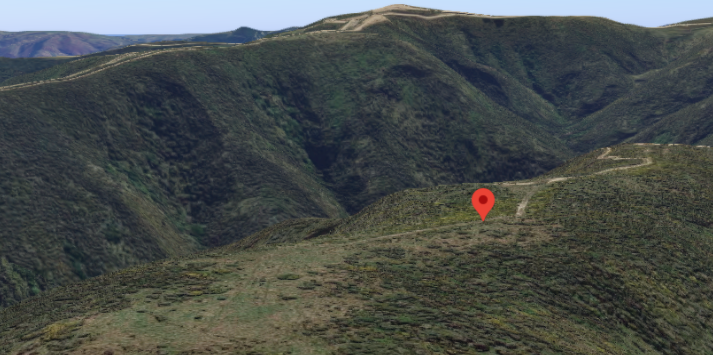
\includegraphics[width=\textwidth]{fig/pin_location.png}
        \label{ap:location}
        \section{Wind Resource}
        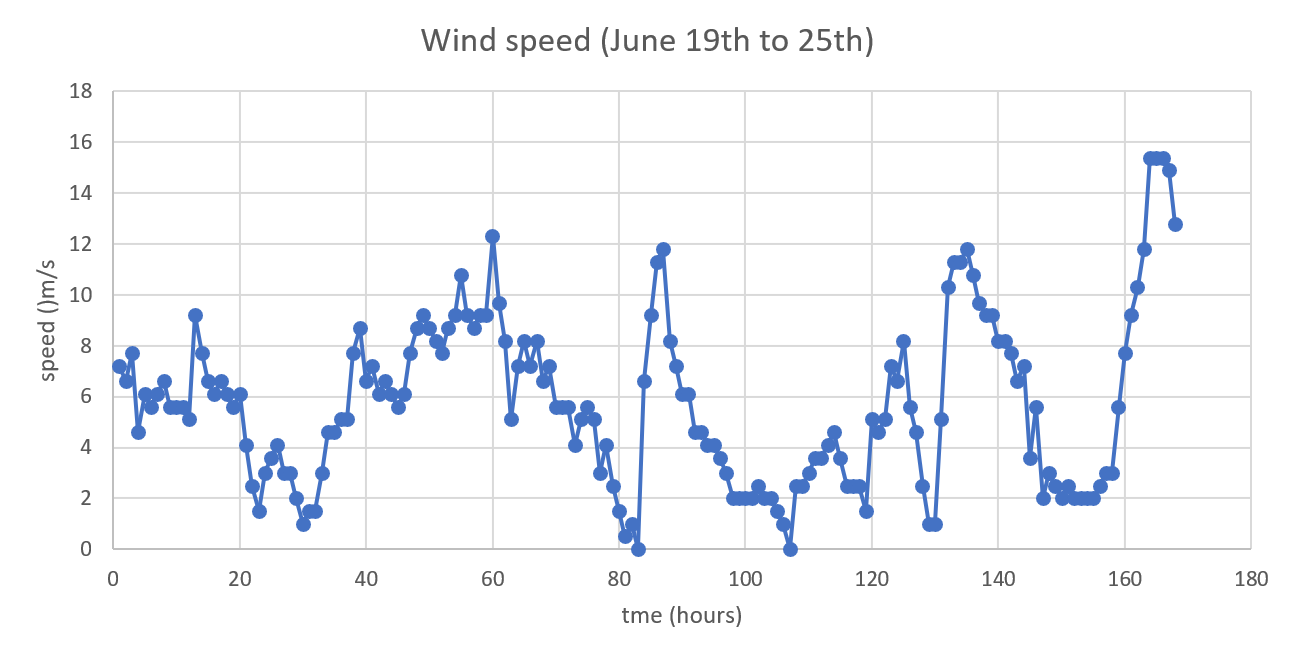
\includegraphics[width=0.5\textwidth]{fig/windspeed.png}
        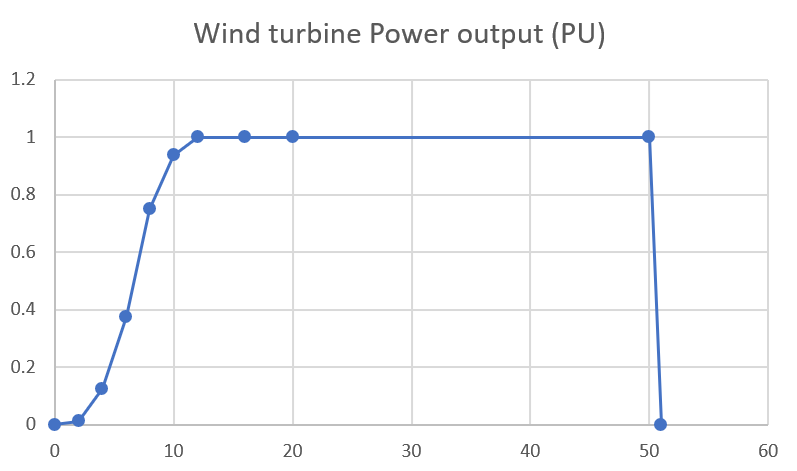
\includegraphics[width=0.5\textwidth]{fig/turbineresp.png}
        \label{ap:wind}

        \section{Models}
        \label{ap:models}
        \begin{center}
                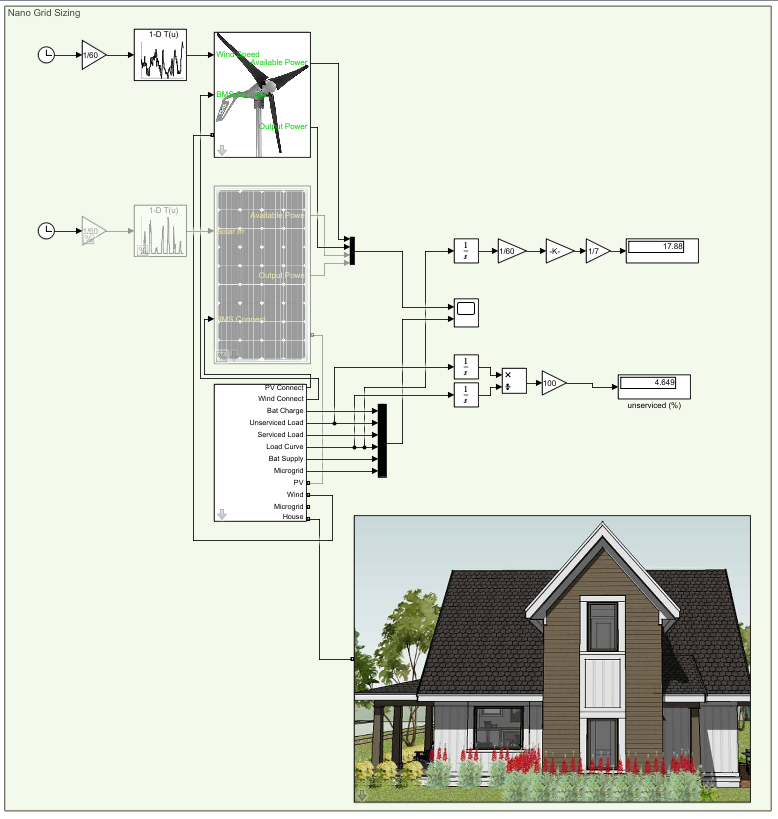
\includegraphics[width=0.5\textwidth]{fig/nano_sim.png}
                
                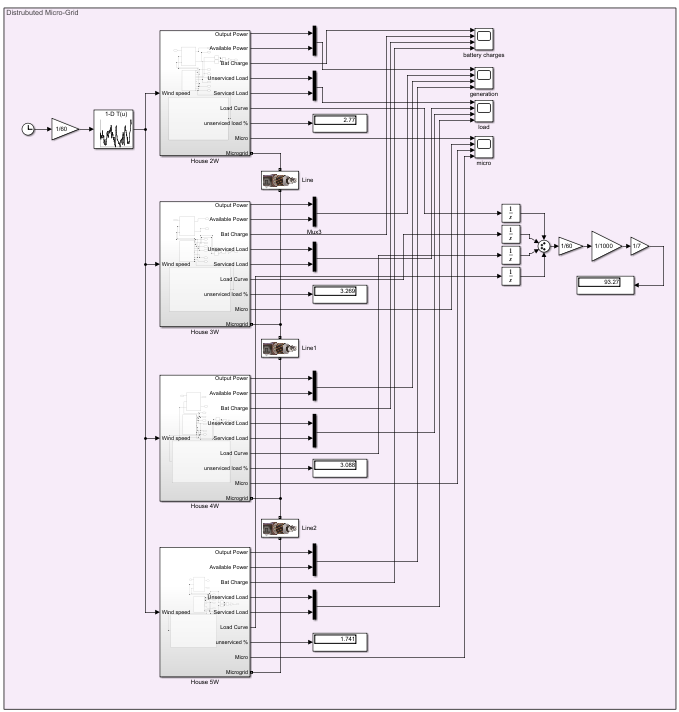
\includegraphics[width=0.5\textwidth]{fig/distrib_sim.png}
                
                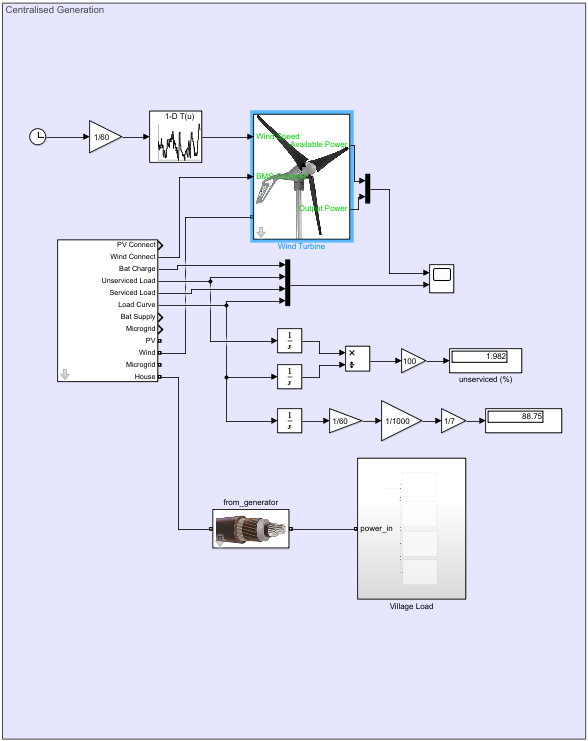
\includegraphics[width=0.5\textwidth]{fig/central_sim.png}
        \end{center}
        



\newpage
\bibliography{ref}
\bibliographystyle{IEEEtran}
\end{document}
